\let\negmedspace\undefined
\let\negthickspace\undefined
\documentclass[journal]{IEEEtran}
\usepackage[a5paper, margin=10mm, onecolumn]{geometry}
%\usepackage{lmodern} % Ensure lmodern is loaded for pdflatex
\usepackage{tfrupee} % Include tfrupee package

\setlength{\headheight}{1cm} % Set the height of the header box
\setlength{\headsep}{0mm}     % Set the distance between the header box and the top of the text

\usepackage{gvv-book}
\usepackage{gvv}
\usepackage{cite}
\usepackage{amsmath,amssymb,amsfonts,amsthm}
\usepackage{algorithmic}
\usepackage{graphicx}
\usepackage{textcomp}
\usepackage{xcolor}
\usepackage{txfonts}
\usepackage{listings}
\usepackage{enumitem}
\usepackage{mathtools}
\usepackage{gensymb}
\usepackage{comment}
%\usepackage{multiclo}
\usepackage[breaklinks=true]{hyperref}
\usepackage{tkz-euclide} 
\usepackage{listings}
% \usepackage{gvv} 
\graphicspath{ {./figs/} }

\begin{document}


\title{
ASSIGNMENT 1: GATE 2007 \\
MN:MINING ENGINEERING}
\author{AI25BTECH11010 - Dhanush Kumar}
\maketitle
\renewcommand{\thefigure}{\theenumi}
\renewcommand{\thetable}{\theenumi}

\begin{enumerate}
    \item If the slope of a diagonal of a rectangle is $m$, the slope of the other diagonal is
	     \hfill (GATE MN 2007)
    \begin{enumerate}
	 \begin{multicols}{4}	    
        \item $\frac{1}{2m}$ 
        \item $-\frac{1}{2m}$
        \item $\frac{1}{m}$
        \item $-\frac{1}{m}$ 
	\end{multicols}	
    \end{enumerate}


    \item If the rank of a matrix $A$ is $r$, the rank of the matrix $A^T$ is
	    \hfill (GATE MN 2007)
	    \begin{enumerate}
    \begin{multicols}{2}	    
        \item $r$, if and only if $A^T = A$
        \item $r$, for all $A$
        \item $p$, where $p \neq r$
        \item $r - 1$, where $r \geq 1$
        \end{multicols}
    \end{enumerate}


    \item Bulk modulus of rock is defined as
	    \hfill (GATE MN 2007)
    \begin{enumerate}
	\begin{multicols}{2}	    
        \item $\frac{\text{shear stress}}{\text{volumetric strain}}$	
        \item $\frac{\text{hydrostatic pressure}}{\text{shear strain}}$
        \item $\frac{\text{hydrostatic pressure}}{\text{volumetric strain}}$	
        \item $\frac{\text{shear stress}}{\text{shear strain}}$
	\end{multicols}	
    \end{enumerate}


    \item The magnitude of the resultant moment about point O in Nm of the two forces acting on the rod shown below is
	    \hfill (GATE MN 2007)
    \begin{figure}[H]
    \centering
        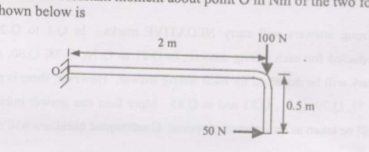
\includegraphics[width=0.7\textwidth]{Screenshot_2025_0812_111906.png}
	    \caption{}
    \label{fig:Q4}
    \end{figure}
    \begin{enumerate}
	\begin{multicols}{4}	    
        \item 25 
        \item 125 
        \item 175 
        \item 225 
	\end{multicols}	
    \end{enumerate}


    \item Radial stress on the excavation boundary of a circular tunnel is
	    \hfill (GATE MN 2007)
    \begin{enumerate}
		    
        \item always zero
        \item always positive
        \item always negative
        \item positive in some area and negative in some area
		
    \end{enumerate}


    \item The critical diameter of an explosive is defined as the diameter below which it
	    \hfill (GATE MN 2007)
    \begin{enumerate}
        \item develops the optimum velocity of detonation
        \item does not involve in chemical reaction
        \item develops the maximum velocity of detonation
        \item deflagrates
		
    \end{enumerate}


    \item Which one of the following supports does NOT require a power pack for its operation
	    \hfill (GATE MN 2007)
    \begin{enumerate}
		    \begin{multicols}{2}
        \item chock shield support
        \item open circuit hydraulic prop
        \item close circuit hydraulic prop
        \item Alpine breaker line support
          \end{multicols}
    \end{enumerate}


    \item In a centrifugal flow fan the conversion of velocity pressure to static pressure is accomplished with the help of
	    \hfill (GATE MN 2007)
\begin{enumerate}
	\begin{multicols}{4}	
    \item impeller
    \item curved blades
    \item hub
    \item casing
	\end{multicols} 

		
\end{enumerate}


   \item A 3.3 kV, 3-phase AC motor having a PF of 0.85 draws current at 95 A. The motor input power in kW is
	   \hfill (GATE MN 2007)
\begin{enumerate}
	\begin{multicols}{4}	
    \item 266.5
    \item 461.5
    \item 543.0
    \item 799.5
	\end{multicols}    
\end{enumerate}


   \item The amount of total stone dust required in kg for a secondary/heavy type stone dust barrier in a roadway of size 4.0 m $\times$ 3.0 m is
	   \hfill (GATE MN 2007)
\begin{enumerate}
		\begin{multicols}{4}
    \item 1320
    \item 4680
    \item 5200
    \item 6600
	    \end{multicols}
\end{enumerate}


\item In the Gaussian plume model, the dispersion coefficients are function of
	\hfill (GATE MN 2007)
\begin{enumerate}
		
    \item distance from source and stability class
    \item stack height and distance from source
    \item stability class and source coordinates
    \item source coordinates and distance from source
	    
\end{enumerate}


\item The rachet-and-pawl arrangement in percussive drill machine helps in
	\hfill (GATE MN 2007)
\begin{enumerate}
		
		
    \item providing required rotational speed
    \item indexing at the bit rock interface
    \item regulating air flow in forward and return strokes of the piston
    \item engaging the bit with the rock between the blows
	    
\end{enumerate}


\item The measurement of distances from a position on the earth to artificial satellites is
	\hfill (GATE MN 2007)
\begin{enumerate}
		
		\begin{multicols}{2}
    \item astronomical ranging
    \item pseudo ranging
    \item satellite ranging
    \item celestial ranging
	    \end{multicols}
\end{enumerate}


\item In opencast mining, the width which is extracted from the working bench is termed as
	\hfill (GATE MN 2007)
\begin{enumerate}
		\begin{multicols}{4}
    \item cut
    \item bench width
    \item bank width
    \item bench face
	    \end{multicols}
\end{enumerate}


\item Zener barriers are associated with
	\hfill (GATE MN 2007)
\begin{enumerate}
		
    \item increased safety apparatus
    \item statistically safe apparatus
    \item flame proof apparatus
    \item intrinsic safety
	    
\end{enumerate}


\item The most recent model of self-contained compressed-oxygen breathing apparatus is
	\hfill (GATE MN 2007)
\begin{enumerate}
		\begin{multicols}{4}
    \item Proto-IV
    \item BG-174
    \item BG-4
    \item BG-174A
	    \end{multicols}
\end{enumerate}



\item The measures of dispersion are
\hfill (GATE MN 2007)
\begin{enumerate}
    \item range, variance, and standard deviation
    \item mean, median, and variance
    \item mean, mode, and skewness
    \item mean, range, and variance

\end{enumerate}


\item In a single server queueing model with constant arrival rate, which one of the following probability distributions is followed by the inter–arrival times of the customers at the service facility?
	\hfill (GATE MN 2007)
\begin{enumerate}
		\begin{multicols}{4}
    \item binomial
    \item Poisson
    \item Weibull
    \item exponential
	    \end{multicols}
\end{enumerate}



\item A company invested Rs.\ 4 lakh in a machine with an expected useful life of 12 years. The net income expected from the operation of the machine is Rs.\ 80,000 per annum. The payback period for the machine in years is
\hfill (GATE MN 2007)	
\begin{enumerate}
		\begin{multicols}{4}
    \item 4
    \item 5
    \item 6
    \item 7
	    \end{multicols}
\end{enumerate}


\item The angular (horizontal/vertical) observation made by a transit theodolite with the face of the vertical circle on the right of the observer is called
	\hfill (GATE MN 2007)
\begin{enumerate}
		\begin{multicols}{2}
    \item face right observation
    \item face left observation
    \item normal observation
    \item reciprocal observation
	    \end{multicols}
\end{enumerate}





\item Two sides of a triangle are represented by vectors $\mathbf{a} = \hat{i} + \hat{j} + \hat{k}$ and $\mathbf{b} = -\hat{i} - \hat{j} + \hat{k}$. The area (magnitude) of the triangle is
\hfill (GATE MN 2007)
\begin{enumerate}
		\begin{multicols}{4}
    \item $\frac{1}{\sqrt{2}}$
    \item 1
    \item $\sqrt{2}$
    \item $2\sqrt{2}$
	    \end{multicols}
\end{enumerate}


\item The cost of diesel is Rs.\ $\left(25 + \frac{x}{90}\right)$ per km to drive a dump truck at a speed of $x$ km/hour. The maintenance cost of the truck is Rs.\ 10 per hour. To minimize the cost per km, the truck speed in km/hour is
	\hfill (GATE MN 2007)
\begin{enumerate}
		\begin{multicols}{4}
    \item 5
    \item 20
    \item 25
    \item 30
	    \end{multicols}
\end{enumerate}



\item The functions $f(x)$ and $g(x)$ satisfy $f(x=0)=3$, $f'(x=0)=-5$, $g(x=0)=2$ and $g'(x=0)=-10$. The value of 
\[
\frac{d}{dx} \left( \frac{f(x)}{g(x)} \right)_{x=0}
\]
is
\hfill (GATE MN 2007)
\begin{enumerate}
		\begin{multicols}{4}
    \item $-35.0$
    \item $-5.0$
    \item $0.5$
    \item $5.0$
	    \end{multicols}
\end{enumerate}



\item A wooden block of 50 kg rests on the floor (shown in figure below) for which the coefficient of static friction is 0.5. The smallest magnitude of the force $P$ in kg that will cause impending motion of the block is
	\hfill (GATE MN 2007)
	\begin{figure}[H]
    \centering
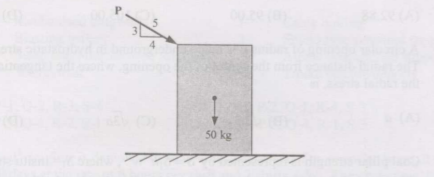
\includegraphics[width=0.4\textwidth]{Screenshot_2025_0812_123307.png}
\caption{}
    \label{fig:Q24}
\end{figure}
\begin{enumerate}
    \begin{multicols}{4}
    \item 50
    \item 40
    \item 30
    \item 25
	    \end{multicols}
\end{enumerate}


\item The solution of $y e^x dx + (4y + e^x) dy = 0$ for $y(0) = -1$ is
	\hfill (GATE MN 2007)
\begin{enumerate}
    \begin{multicols}{2}
    \item $y e^x + 2y^2 - 1 = 0$
    \item $e^x + y^2 - 2 = 0$
    \item $y e^x - y^2 = 0$
    \item $y e^x + y^2 - 1 = 0$
	    \end{multicols}
\end{enumerate}


\item A point $P(10,3)$ MPa on the Mohr’s circle represents normal and shear stresses. If the centre of the Mohr’s circle is $C(6,0)$ MPa, the normal and shear stresses in MPa on the point diametrically opposite to $P$ are
	\hfill (GATE MN 2007)
\begin{enumerate}
	\begin{multicols}{4}
    \item 2, $-3$
    \item 4, $-3$
    \item 2, 3
    \item 4, 3
	    \end{multicols}
\end{enumerate}


\item A rock sample with a horizontal joint is subjected to 10 MPa of normal pressure as shown in the figure. The elastic modulus and Poisson’s ratio of the rock are 5.0 GPa and 0 respectively. If the normal stiffness ($k_n$) of the joint is 50 GPa/m, normal displacement at the top of the sample (A$A'$ line) in mm is
	\hfill (GATE MN 2007)
\begin{figure}[H]
    \centering
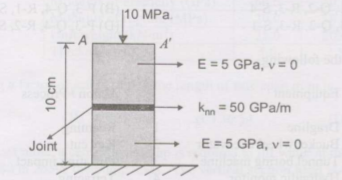
\includegraphics[width=0.35\textwidth]{Screenshot_2025_0812_124013.png}
\caption{}
    \label{fig:Q27}
\end{figure}
\begin{enumerate}
	\begin{multicols}{4}
    \item 0.2
    \item 0.4
    \item 0.6
    \item 0.8
	    \end{multicols}
\end{enumerate}



\item The state of stress $(\sigma_{xx}, \sigma_{yy}, \tau_{xy})$ at a point below ground is found to be $(5, 15, -3)$ MPa. The angle measured in the counter clockwise direction between the x-axis and the major principal axis in degree is
	\hfill (GATE MN 2007)
\begin{enumerate}
		\begin{multicols}{4}
    \item 9.52
    \item 15.48
    \item 150.48
    \item 164.52
	    \end{multicols}
\end{enumerate}


\item The unconfined compressive strength of a cylindrical rock sample is 90 MPa. The angle of internal friction of the rock is $30^\circ$. If a confining pressure of 5 MPa is applied radially to the rock sample, the confined compressive strength in MPa is
	\hfill (GATE MN 2007)
\begin{enumerate}
		\begin{multicols}{4}
    \item 92.88
    \item 95.00
    \item 105.00
    \item 110.0
	    \end{multicols}
\end{enumerate}



\item A circular opening of radius $a$ is made underground in hydrostatic stress condition. The radial distance from the centre of the opening, where the tangential stress is twice the radial stress, is
\hfill (GATE MN 2007)
\begin{enumerate}
		\begin{multicols}{4}
\item $a$
\item $\sqrt{2}a$
\item $\sqrt{3}a$
\item $2\sqrt{3}a$
	\end{multicols}
\end{enumerate}



\item Coal pillar strength is represented by $S = S_{in} h^\alpha w^\beta$, where $S_{in}$ = insitu strength of the pillar, $h$ = mining height, and $w$ = pillar width. Two bord and pillar panels are developed in the similar geological conditions at depths $D_1$ and $D_2$ with mining heights $h_1$ and $h_2$ respectively. If the gallery width and the pillar width in both the panels remain the same, the ratio of pillar safety factors, $SF_1/SF_2$ is
\hfill (GATE MN 2007)
\begin{enumerate}
		\begin{multicols}{4}
\item $\left(\frac{h_2}{h_1}\right)^\alpha \frac{D_1}{D_2}$
\item $\left(\frac{h_2}{h_1}\right)^\alpha \frac{D_2}{D_1}$
\item $\left(\frac{h_1}{h_2}\right)^\alpha \frac{D_2}{D_1}$
\item $\left(\frac{h_1}{h_2}\right)^\alpha \frac{D_1}{D_2}$
	\end{multicols}
\end{enumerate}



\item Match the following
\begin{table}[H]
    \centering\normalsize
\begin{tabular}{llcl}
\multicolumn{2}{l}{\textbf{Belt conveyor component}} & & \textbf{Function} \\
P & Pull cord      &  & 1. Cleaning device \\
Q & Snub pulley    &  & 2. Discharging material side of the conveyor \\
R & Tripper        &  & 3. Safety stopping device \\
S & Rotary brush   &  & 4. Increasing the angle of wrap \\
\end{tabular}
\caption{}
    \label{tab:Q32}
\end{table}

\hfill (GATE MN 2007)

\begin{enumerate}
		\begin{multicols}{2}
\item P-1, Q-2, R-3, S-4
\item P-3, Q-4, R-1, S-2
\item P-4, Q-2, R-3, S-1
\item P-3, Q-4, R-2, S-1
	\end{multicols}
\end{enumerate}




\item Match the following
\begin{table}[H]
    \centering\normalsize
\begin{tabular}{llcl}                             
\multicolumn{2}{l}{\textbf{Equipment  }} & & \textbf{Action/Process} \\
P & Dragline       &  & 1. Reaming \\ 
Q & Bucket wheel excavator    &  & 2. Key cut \\                     
R & Tunnel boring machine   &  & 3. Pulsatng impact    \\                                                
S & Hydraulic monitor   &  & 4. Terracing \\                                       
\end{tabular}
\caption{}
    \label{tab:Q33}
\end{table}
\hfill (GATE MN 2007)
\begin{enumerate}
		\begin{multicols}{2}
\item P-1, Q-2, R-3, S-4
\item P-2, Q-4, R-1, S-3
\item P-2, Q-4, R-3, S-1
\item P-3, Q-4, R-2, S-1
	\end{multicols}
\end{enumerate}



\item Match the following
\begin{table}[H]
    \centering\normalsize
\begin{tabular}{llcl}                             
\multicolumn{2}{l}{\textbf{Mining method    }} & & \textbf{Face supporting system} \\                       
P & Mechanised longwall     &  & 1. Cable bolting \\     
Q & Blasting gallery    &  & 2. Shield type powered supports \\                         
R & Steep seam mechanised longwall        &  & 3.Alpine breaker line supports     \\                                               
S & Wangawilli   &  & 4. troika shield supports \\                                          
\end{tabular}
\caption{}
    \label{tab:Q34}
\end{table}
\hfill (GATE MN 2007)
\begin{enumerate}
		\begin{multicols}{2}
\item P-1, Q-2, R-3, S-4
\item P-2, Q-1, R-4, S-3
\item P-3, Q-4, R-2, S-1
\item P-2, Q-4, R-1, S-3
	\end{multicols}
\end{enumerate}



\item A $15 \ \text{yd}^3$ dragline is deployed in an overburden bench of an opencast mine. It works for 40 days at the rate of 6 hours per shift and 3 shifts a day. The cycle time, bucket fill factor, and operating efficiency of the dragline are respectively 50 s, 0.8, and 75\%. The total volume of overburden in m$^3$ handled by the dragline is \\
(1 yd$^3$ = 0.765 m$^3$)

\hfill (GATE MN 2007)
\begin{enumerate}
		\begin{multicols}{4}
\item 356918
\item 634521
\item 557685
\item 991440
	\end{multicols}
\end{enumerate}



\item The phenomenon of fretting (necking) of pillars in room-and-pillar stoping is common in the pillars formed in
	\hfill (GATE MN 2007)
\begin{enumerate}
\item massive rock with very high pillar height to width ratio
\item regularly jointed rock with high pillar height to width ratio
\item massive rock with low pillar height to width ratio
\item transversely jointed rock with low pillar height to width ratio
\end{enumerate}
\item In an underground opening, the immediate roof strata consists of two rock layers with the following properties:

\begin{table}[H]
    \centering\normalsize
\begin{tabular}{|l|c|c|}
\hline
Property & Layer-1 & Layer-2 \\
\hline
Modulus of elasticity (GPa) & 60.0 & 40.0 \\
\hline
Modulus of rupture (MPa) & 20.0 & 10.0 \\
\hline
Unit weight (kN/m$^3$) & 25.0 & 20.0 \\
\hline
Thickness (m) & 2.5 & 2.5 \\
\hline
\end{tabular}
\caption{}
    \label{tab:Q37}
\end{table}

Considering a factor of safety of 4.0, the length of safe span in m is
\hfill (GATE MN 2007)
\begin{enumerate}
		\begin{multicols}{4}
\item 27.82
\item 34.06
\item 36.54
\item 39.34
	\end{multicols}
\end{enumerate}


\item In an opencast mine, a centrifugal pump is required to lift water at the rate of 60 l/s to a height of 80 m above the pump level. The vertical suction head is 4 m. The total friction head including shock and energy loss is 10 m. If the pump runs at an efficiency of 80\%, the brake power of the motor in kW is
	\hfill (GATE MN 2007)
\begin{enumerate}
		\begin{multicols}{4}
\item 70.50
\item 67.50
\item 63.00
\item 57.55
	\end{multicols}
\end{enumerate}



\item Match the following:
\begin{table}[H]
    \centering\normalsize
\begin{tabular}{p{5cm} p{5cm}}
\textbf{Support system} & \textbf{Support principle} \\
P \quad Shotcrete & 1 \quad reinforces rock mass by binding them together \\
Q \quad Backfill & 2 \quad acts as link between two layers of rock to transfer load between them \\
R \quad Bolt & 3 \quad imposes kinematic constraints on key pieces in a stope boundary \\
S \quad Prop & 4 \quad prevents spatially progressive disintegration of near field rock mass \\
\end{tabular}
 \caption{}
    \label{tab:Q39}
\end{table}
\hfill (GATE MN 2007)
\begin{enumerate}
		\begin{multicols}{2}
\item P-3, Q-4, R-2, S-1
\item P-2, Q-1, R-4, S-2
\item P-4, Q-3, R-1, S-2
\item P-3, Q-4, R-1, S-2
	\end{multicols}
\end{enumerate}


\item Match the following:
\begin{table}[H]
    \centering\normalsize
\begin{tabular}{p{3cm} p{4cm} p{6cm}}
\textbf{Stope} & \textbf{Drill machine} & \textbf{Method of drilling} \\
P \quad Shrinkage & I \quad Drill jumbo & 1 \quad Fan drilling \\
Q \quad Room-and-pillar & J \quad Down-the-hole hammer & 2 \quad Overhand drilling \\
R \quad Sublevel & K \quad Hand held stopper & 3 \quad Parallel drilling \\
S \quad Sublevel caving & L \quad Mechanised fan drill & 4 \quad Frontal/vertical/downward benching \\
\end{tabular}
 \caption{}
    \label{tab:Q40}
\end{table}
\hfill (GATE MN 2007)
\begin{enumerate}
		\begin{multicols}{2}
\item P-I-2, Q-K-4, R-L-3, S-J-1
\item P-K-4, Q-I-3, R-J-2, S-L-1
\item P-K-2, Q-L-4, R-J-3, S-I-1
\item P-I-3, Q-K-4, R-J-1, S-L-2
	\end{multicols}
\end{enumerate}



\item A coal seam of 12 m thickness is worked out by mechanized top coal caving system. The thickness of the bottom slice is 3 m, length of the solid coal face is 120 m and the average depth of cut by the shearer (web) is 70 cm. The density of coal is 1300 kg/m$^3$ with the percentage of extraction in the slice at 95 and in the top coal at 70. The production of coal per cycle in tonne is 
	\hfill (GATE MN 2007)
\begin{enumerate}
       \begin{multicols}{4}
    \item 1008
    \item 999
    \item 688
    \item 311
	    \end{multicols}
\end{enumerate}


\item Two reservoirs are connected by two equal length parallel pipelines with diameters $d$ and $2d$. Assuming similar resistance coefficients, if the discharge through the smaller diameter pipeline is 0.04 m$^3$/s, the discharge through the other pipeline in m$^3$/s is 
	\hfill (GATE MN 2007)
\begin{enumerate}
       \begin{multicols}{4}
    \item 0.226
    \item 0.426
    \item 1.130
    \item 1.280
	    \end{multicols}
\end{enumerate}


\item The shear force diagram for the shaft shown below resembles which one of the following graphs?  

\begin{figure}[H]
    \centering
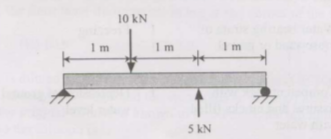
\includegraphics[width=0.6\textwidth]{Screenshot_2025_0812_143315.png}
\caption{}
    \label{fig:Q43}
\end{figure}
\hfill (GATE MN 2007)
\begin{multicols}{2}
	Graph-I \\
	\begin{figure}[H]
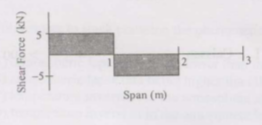
\includegraphics[width=0.45\textwidth]{Screenshot_2025_0812_143545.png} \\
\caption{}
\label{fig:Q43option1}
 \end{figure}
Graph-II \\
\begin{figure}[H]
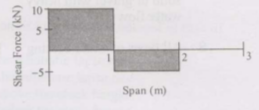
\includegraphics[width=0.45\textwidth]{Screenshot_2025_0812_143610.png} \\
\caption{}
  \label{fig:Q43option2}
  \end{figure}
Graph-III \\
\begin{figure}[H]
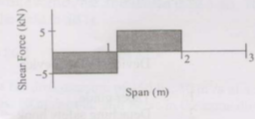
\includegraphics[width=0.45\textwidth]{Screenshot_2025_0812_144908.png} \\
\caption{}
  \label{fig:Q43option3}
  \end{figure}
Graph-IV \\
\begin{figure}[H]
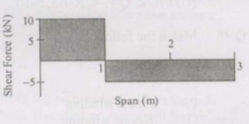
\includegraphics[width=0.45\textwidth]{Screenshot_2025_0812_143638.png} \\
\caption{}
\label{fig:Q43option4}
 \end{figure}
\end{multicols}
\begin{enumerate}                               
\begin{multicols}{4}            
\item Graph-I                                 
\item Graph-II                                
\item Graph-III                              
\item Graph-IV                                  
\end{multicols}                                  
\end{enumerate}


\item A 12 tonne diesel locomotive of 60 kW is plying in an underground haulage roadway. The coefficient of adhesion is 0.25 and the maximum gear efficiency is 80\%. The speed in m/s at which it will haul a train at its full power is 
	\hfill (GATE MN 2007)
\begin{enumerate}
		\begin{multicols}{4}
    \item 2.548
    \item 2.448
    \item 2.038
    \item 1.630
\end{multicols}
\end{enumerate}


\item An air receiver of volume 0.2 m$^3$ has an initial temperature of 27$^\circ$C and pressure 1800 kPa. After use, the air pressure falls to 1200 kPa at a temperature of 17$^\circ$C. The volume of air consumed in m$^3$ corresponding to an air pressure of 101.3 kPa and temperature of 0$^\circ$C is  
	\hfill (GATE MN 2007)
\begin{enumerate}
     \begin{multicols}{4}
    \item 0.693
    \item 0.895
    \item 1.002
    \item 1.251
	    \end{multicols}
\end{enumerate}


\item Four benches are being worked by the opencast mining system. Height, width and face angle for each bench are 15 m, 50 m and 70$^\circ$ respectively. The overall slope angle of the benches in degrees is  
	\hfill (GATE MN 2007)
\begin{enumerate}
   \begin{multicols}{4}
    \item 15.45
    \item 19.25
    \item 32.65
    \item 36.25
	    \end{multicols}
\end{enumerate}


\item Match the following
\begin{table}[H]
    \centering\normalsize
\begin{tabular}{p{4.5cm} p{4.5cm} p{4cm}}
\textbf{Rock mass condition} & \textbf{Shaft sinking method} & \textbf{Limiting depth (m)} \\
P: Water bearing strata of loose sand or gravel & I: Freezing & 1: 40 \\
Q: Competent rock with fissures and cracks filled with water & J: Depression of ground water level & 2: 150 \\
R: Highly permeable coarse solid or gravel with heavy water flow & K: Cement grouting & 3: 1000 \\
S: All types of water bearing rocks & L: Caisson & 4: $>$600 \\
\end{tabular}
\caption{}
    \label{tab:Q47}
\end{table}
\hfill (GATE MN 2007)
\begin{enumerate}
		\begin{multicols}{2}
\item P-L-4, Q-K-1, R-J-2, S-I-3
\item P-L-1, Q-K-4, R-J-2, S-I-3
\item P-L-2, Q-K-4, R-J-3, S-I-1
\item P-L-4, Q-K-3, R-J-2, S-I-1
	\end{multicols}
\end{enumerate}


\item Match the following
\begin{table}[H]
    \centering\normalsize
\begin{tabular}{p{4.5cm} p{6cm}}
\textbf{System} & \textbf{Device / Safety device} \\
P: Drum winding & 1: Taper guide \\
Q: Koepe winding & 2: Detaching safety hook \\
R: Inclined Haulage & 3: Rider \\
S: Winding in sinking shaft & 4: Back catch \\
\end{tabular}
\caption{}
    \label{tab:Q48}
\end{table}
\hfill (GATE MN 2007)
\begin{enumerate}
    \begin{multicols}{2}
\item P-1, Q-2, R-3, S-4
\item P-4, Q-3, R-1, S-2
\item P-2, Q-1, R-3, S-4
\item P-2, Q-1, R-4, S-3
	\end{multicols}
\end{enumerate}


\item A closed container with 10 kg of air at ambient pressure and specific heat 1020 kJ/kg$^\circ$C is cooled from 35$^\circ$C. If the removal of 200 kJ of heat resulted in the saturation of air, the corresponding dew point temperature in $^\circ$C is:
\hfill (GATE MN 2007)
\begin{enumerate}
		\begin{multicols}{4}
\item 33.0
\item 27.3
\item 15.4
\item 12.9
	\end{multicols}
\end{enumerate}


\item Identify the \textbf{INCORRECT} statement
\hfill (GATE MN 2007)
\begin{enumerate}
\item Evasee is meant to minimise exit shock losses
\item Evasee efficiency is primarily a function of divergence angle and area ratio
\item Evasee produces an inevitable increase in friction losses
\item Evasee installation leads to reduction in the fan total pressure
\end{enumerate}


\item A single lamp placed centrally at the roof provides 40 lux illumination vertically below, at the floor of an underground workshop. The workshop is of dimensions 20.0 m $\times$ 20.0 m with height 4.0 m. Assuming uniform spherical dispersion of luminous intensity, the floor level illumination in lux at any corner of the workshop is:
\hfill (GATE MN 2007)
\begin{enumerate}
\begin{multicols}{4}
\item 23.2
\item 10.9
\item 3.0
\item 0.8
	\end{multicols}
\end{enumerate}


\item An effluent sample is diluted with fresh water to make up a solution of 300 ml. The DO of the solution initially is 8.0 mg/l and the value falls to 3.0 mg/l after 5 days. If the 5-day BOD of the original effluent is known to be 50 mg/l, the amount of fresh water added in ml to the solution is:
\hfill (GATE MN 2007)
\begin{enumerate}
		\begin{multicols}{4}
\item 270
\item 160
\item 54
\item 30
	\end{multicols}
\end{enumerate}



\item With respect to stack emission the phenomenon of fumigation is noticed in case of 
	\hfill (GATE MN 2007)
\begin{enumerate}
    \item atmospheric lapse rate being lower than the adiabatic lapse rate
    \item atmospheric lapse rate being higher than the adiabatic lapse rate
    \item temperature inversion in the atmosphere above the stack height
    \item temperature inversion in the atmosphere below the stack height
\end{enumerate}


\item A jackhammer operates at a corner of a square field of side $50\,\text{m}$.  
At the diagonally opposite corner, the SPL sensed is $82.3\,\text{dB}$.  
The SPL at any of the other two corners of the field in dB is  
\hfill (GATE MN 2007)
\begin{enumerate}
		\begin{multicols}{4}
    \item 86.3
    \item 85.3
    \item 83.6
    \item 81.2
	    \end{multicols}
\end{enumerate}



\item At a fan drift pressure of $450\,\text{Pa}$, $50\,\text{m}^3/\text{s}$ of air flows through a mine.  
When the fan stops, $10\,\text{m}^3/\text{s}$ of air still flows in the same direction.  
The mine resistance in Ns$^2$/m$^8$ is
\hfill (GATE MN 2007)
\begin{enumerate}
		\begin{multicols}{4}
    \item 0.1731
    \item 0.1800
    \item 0.1875
    \item 0.2372
	    \end{multicols}
\end{enumerate}


\item In an experiment to determine rock thermal conductivity,a disc of rock specimen is placed between two solid brass cylinders and one-dimensional heat flow is created as shown in the figure.  
The readings of the thermocouple sensors with respect to zero potential are shown in the figure.  
Brass thermal conductivity is $90\,\text{W/m$^\circ$C}$, and the thermocouple constant is $40\,\mu\text{V}/^\circ$C.  
\hfill (GATE MN 2007)
\begin{figure}[H]
    \centering
    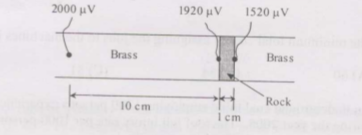
\includegraphics[width=0.6\textwidth]{Screenshot_2025_0812_172517.png}
\caption{}
    \label{fig:Q56}
\end{figure}

The rock thermal conductivity in W/m$^\circ$C and the heat flux in W/m$^2$ respectively are  
\begin{enumerate}
\begin{multicols}{4}
    \item 1.8, 1800
    \item 0.6, 1020
    \item 3.2, 540
    \item 2.1, 670
	    \end{multicols}
\end{enumerate}


\item Consider the following data for the grade of iron ore from a working bench over past 5 weeks:
\hfill (GATE MN 2007)
\begin{table}[H]
    \centering\normalsize
\begin{tabular}{|c|c|}
\hline
Week & Grade (\% Fe) \\
\hline
1 & 62.1 \\
\hline
2 & 61.0 \\
\hline
3 & 60.5 \\
\hline
4 & 62.5 \\
\hline
5 & 62.0 \\
\hline
\end{tabular}
   \caption{}
    \label{tab:Q57}
\end{table}

The 3-week moving average forecast for the grade, in \% Fe, in the 6th week is:
\hfill (GATE MN 2007)
\begin{enumerate}
   \begin{multicols}{4}
    \item 61.66
    \item 61.90
    \item 62.20
    \item 62.50
	    \end{multicols}
\end{enumerate}


\item The random variable $X$ has the following probability mass function:  
\[
P(4) = \frac14, \quad P(8) = \frac14, \quad P(12) = \frac14, \quad P(16) = \frac14
\]
The expected value of $X$ is:  
\hfill (GATE MN 2007)
\begin{enumerate}
\begin{multicols}{4}
    \item 1
    \item 3
    \item 10
    \item 12
	    \end{multicols}
\end{enumerate}


\item The time between successive failures (in hours) of a side discharge loader operating in a mechanised underground coal mine are as follows:  
\[
62, \; 58, \; 54, \; 50, \; 52, \; 60, \; 58, \; 57, \; 50, \; 53
\]
If the failure data follow an exponential distribution, then reliability of the equipment for a period of 50 hours is: 
\hfill (GATE MN 2007)
\begin{enumerate}
\begin{multicols}{4}
    \item 0.25
    \item 0.40
    \item 0.60
    \item 1.00
	    \end{multicols}
\end{enumerate}


\item Three jobs A, B, and C are to be assigned to three machines X, Y and Z. The processing costs are given below:

\begin{table}[ht]
\centering
\renewcommand{\arraystretch}{1.2}
\begin{tabular}{|c|c|c|c|c|}
\hline
\multicolumn{2}{|c|}{} & \multicolumn{3}{c|}{\textbf{Machine}} \\ \hline
\multirow{3}{*}{\rotatebox{90}{\textbf{Job}}} & A & 19 & 28 & 31 \\ \cline{2-5}
 & B & 11 & 17 & 16 \\ \cline{2-5}
 & C & 12 & 15 & 13 \\ \hline
\end{tabular}
    \caption{}
    \label{tab:Q60}
\end{table}



The minimum total cost of assigning the jobs to the machines is  
\hfill (GATE MN 2007)
\begin{enumerate}
\begin{multicols}{4}
\item 60
\item 54
\item 51
\item 49
\end{multicols}
\end{enumerate}


\item An underground coal mine employing 1200 persons experienced 12 roof fall injuries during the year 2005. The roof fall injury rate per 1000 persons employed during the period 2005, as per the DGMS norms, is  
	\hfill (GATE MN 2007)
\begin{enumerate}
\begin{multicols}{4}
\item 6
\item 8
\item 10
\item 12
	\end{multicols}
\end{enumerate}


\item Consider the following linear programming problem:  
Maximize $Z = 6X_1 + 4X_2$  
Subject to
\[
\begin{aligned}
2X_1 &\le 8, \\
2X_2 &\le 12, \\
3X_1 + 2X_2 &\le 18, \\
X_1 &\ge 0, \ X_2 \ge 0
\end{aligned}
\]
The multiple optimal solutions lie on the line joining the corner points 
\hfill (GATE MN 2007)
\begin{enumerate}
\begin{multicols}{4}
\item (0, 0), (0, 6)
\item (0, 6), (2, 6)
\item (2, 6), (4, 3)
\item (4, 3), (4, 0)
\end{multicols}

\end{enumerate}


\item Match the following:\\
	\begin{table}[H]
    \centering\normalsize
\begin{tabular}{p{4.5cm} p{6cm}}                
\textbf{Problem} & \textbf{Technique}      \\                                              
P:Queuing & 1: Time series models \\            
Q: Project scheduling and monitoring & 2:Linear programming models \\  
R:Transportation & 3:Waiting line models \\     
S: Forecasting of production & 4: PERT and CPM \\
\end{tabular}
    \caption{}
    \label{tab:Q63}
\end{table}
	
\hfill (GATE MN 2007)
\begin{enumerate}
\begin{multicols}{2}
\item P-3, Q-4, R-2, S-1
\item P-2, Q-3, R-4, S-1
\item P-3, Q-4, R-1, S-2
\item P-2, Q-4, R-3, S-1
	\end{multicols}
\end{enumerate}


\item The net present value in Rs. of a 3-year annuity of Rs. 10,000 discounted at 10\% is  
	\hfill (GATE MN 2007)
\begin{enumerate}
		\begin{multicols}{4}
\item 9,091
\item 17,355
\item 24,869
\item 26,446
	\end{multicols}
\end{enumerate}


\item For a track gauge of 1.05 m and a speed of 10 km/hour, the super-elevation in cm from the following figure is
	\begin{figure}[H]
    \centering
	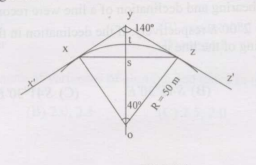
\includegraphics[width=0.4\textwidth]{Screenshot_2025_0812_180648.png}
	\caption{}
    \label{fig:Q65}
\end{figure}

\hfill (GATE MN 2007)
\begin{enumerate}
\begin{multicols}{4}
\item 1.65
\item 2.76
\item 5.54
\item 6.64
	\end{multicols}
\end{enumerate}


\item In the bubble tube of a dumpy level, the bubble moves $5 \ \mathrm{mm}$ for a change of inclination of $40''$. The sensitivity in mm and the radius of the bubble tube in m are \\
($1 \ \mathrm{radian} = 206265''$) \\
\hfill (GATE MN 2007)
\begin{enumerate}
\begin{multicols}{4}
    \item 0.125, 12.89
    \item 0.063, 26.78
    \item 0.125, 25.78
    \item 0.063, 12.89
	    \end{multicols}
\end{enumerate}


\item The value of $A \cdot B$, if 
\[
\vec{A+B}=\myvec{1 & -1 \\ 3 & 0}
\quad \text{and} \quad
\vec{A-B}= \myvec{ 3 & 1 \\ 1 & 4 }
\]
is
\hfill (GATE MN 2007)
\begin{enumerate}
		\begin{multicols}{2}
		\item $-4$$\myvec{1 & 1 \\ 0 & 3}$
    \item $-2$$\myvec{ -2 & 1 \\ 0 & 3}$
    \item $\myvec{ 1 & 3 \\ 1 &1}$
    \item$-\frac{1}{2}$$\myvec{ -2 & 1 \\ 0 & 3 }$
		    \end{multicols}
\end{enumerate}


\item The values of $f(x)$ at $x_0, x_1$ and $x_2$ are 9.0, 12.0 and 15.0 respectively. Using Simpson's $\frac{1}{3}$ rule, the value of $\int f(x) \, dx$, considering an interval of $0.1$ is:
	\hfill (GATE MN 2007)
\begin{enumerate}
		\begin{multicols}{4}
    \item 1.2
    \item 2.4
    \item 1.6
    \item 1.8
	    \end{multicols}
\end{enumerate}


\item From the following page of a levelling field book, the missing values in F.S. and B.S. respectively are:

\begin{table}[H]
    \centering\normalsize
\begin{tabular}{|c|c|c|c|c|c|l|}
\hline
Station & B.S. & I.S. & F.S. & Rise & Fall & Remarks \\
\hline
1 & 4.550 &     &     &      &      & Starting Point \\
\hline
2 & 2.125 &     &     &  ?    & 0.750 & Change point \\
\hline
3 &       & 2.225 &     &      &      &  \\
\hline
4 &    ?   &     & 1.975 &      &      & Change point \\
\hline
5 &       & 2.445 & 1.500 &      &      &  \\
\hline
\end{tabular}
    \caption{}
    \label{tab:Q69}
\end{table}
\hfill (GATE MN 2007)
\begin{enumerate}
\begin{multicols}{4}
    \item 3.804, 0.945
    \item 3.804, 3.945
    \item 5.300, 0.945
    \item 5.300, 3.945
	    \end{multicols}
\end{enumerate}


\item The magnetic bearing and declination of a line were recorded in the year 1906 as $S43^\circ 30' E$ and $2^\circ 00'$ E respectively. If the declination in the year 2000 is $3^\circ 00'$ W, the magnetic bearing of the line is:
	\hfill (GATE MN 2007)
\begin{enumerate}
		\begin{multicols}{4}
    \item $S48^\circ 30' E$
    \item $S45^\circ 30' E$
    \item $S41^\circ 30' E$
    \item $S38^\circ 30' E$
	    \end{multicols}
\end{enumerate}


\begin{center}
	\textbf{Common Data Question}
\end{center}

\textbf{Common Data for Questions 71, 72, 73:}  
In a straight duct of length $200 \, \text{m}$ a fan operates $50 \, \text{m}$ away from the inlet such that the mean air velocity in the duct is $8.0 \, \text{m/s}$ at a density of $1.1 \, \text{kg/m}^3$. The friction pressure loss per m length of the duct is $3.0 \, \text{Pa}$ and the entry shock factor is $1.2$. Answer the following in terms of gauge pressure values in Pa.

    \item The total pressure at the outlet of the duct is 
	    \hfill (GATE MN 2007)
	    \begin{enumerate}
\begin{multicols}{4}
        \item $-35.2$
        \item $35.2$
        \item $192.2$
        \item $635.2$
		\end{multicols}
    \end{enumerate}


    \item The total pressure at the inlet side of the fan is  
	    \hfill (GATE MN 2007)
    \begin{enumerate}
\begin{multicols}{4}
        \item $-192.2$
        \item $-150.0$
        \item $150.0$
        \item $192.2$
		\end{multicols}
    \end{enumerate}

    \item The total pressure generated by the fan is  
	    \hfill (GATE MN 2007)
    \begin{enumerate}
		    \begin{multicols}{4}
        \item $600.0$
        \item $635.2$
        \item $677.4$
        \item $682.2$
		\end{multicols}
    \end{enumerate}


\textbf{Common Data for Questions 74, 75:}  
A bauxite deposit has been intersected by 5 drill holes. The values of alumina (\% by weight) and silica (\% by weight) in these drill holes are as follows:

\begin{table}[H]
    \centering\normalsize
\begin{tabular}{|c|c|c|}
\hline
Drill hole number & Alumina (\%) & Silica (\%) \\
\hline
1 & 46 & 1 \\
\hline
2 & 42 & 5 \\
\hline
3 & 45 & 2 \\
\hline
4 & 43 & 4 \\
\hline
5 & 44 & 3 \\
\hline
\end{tabular}
    \caption{}
    \label{tab:Q74&Q75}
\end{table}

    \item The relationship between alumina and silica is  
	    \hfill (GATE MN 2007)
    \begin{enumerate}
\begin{multicols}{4}
        \item positive linear
        \item exponential
        \item negative linear
        \item random
		\end{multicols}
    \end{enumerate}

    \item The unbiased estimate of variances of alumina and silica in (\%)$^2$ respectively are  
	    \hfill (GATE MN 2007)
    \begin{enumerate}
		    \begin{multicols}{4}
        \item $2.5,\, 2.5$
        \item $2.0,\, 2.5$
        \item $2.5,\, 2.0$
        \item $2.0,\, 2.0$
		\end{multicols}
    \end{enumerate}


\begin{center}
	\textbf{Linked Answer Question}
\end{center}

\textbf{Statement for Linked Answer Questions 76 \& 77:}  
Porosity of a coarse grain sandstone sample is $15\%$. The specific gravity of sandstone is $2.8$.

\item What is the void ratio in the sandstone sample? 
	\hfill (GATE MN 2007)
    \begin{enumerate}
		    \begin{multicols}{4}
        \item $0.150$
        \item $0.176$
        \item $0.850$
        \item $1.176$
		\end{multicols}
    \end{enumerate}


    \item If the sandstone sample is fully saturated in water, the saturated density of the sample in kg/m$^3$ is  
	    \hfill (GATE MN 2007)
    \begin{enumerate}
		    \begin{multicols}{4}
        \item $1590$
        \item $2234$
        \item $2438$
        \item $2531$
		\end{multicols}
    \end{enumerate}



\textbf{Statement for Linked Answer Questions 78 \& 79:} A double outboard chain stranded conveyor is installed in an underground coal mine to transport coal. 
The mass of the chain and associated flight is $40 \ \mathrm{kg/m}$, the coefficients of kinematic friction are $0.33$ between chain and the pan and $0.5$ between conveyed coal and the pan. 
The motor efficiency is $80\%$. 
Coal is to be conveyed at the rate of $120 \ \mathrm{t/hour}$ over a length of $120 \ \mathrm{m}$ at a chain speed of $0.9 \ \mathrm{m/s}$. 
The bulk density of coal is $900 \ \mathrm{kg/m^3}$.
\item The power requirement of the motor of the chain conveyor in kW is  
	\hfill (GATE MN 2007)
\begin{enumerate}
		\begin{multicols}{4}
\item 33.16
\item 37.53
\item 42.00
\item 45.94
	\end{multicols}
\end{enumerate}


\item The power requirement of the motor of the chain conveyor in kW, if it moves in the uphill direction at a gradient of 1 in 10, is 
	\hfill (GATE MN 2007)
\begin{enumerate}
\begin{multicols}{4}
\item 46.91
\item 42.00
\item 38.53
\item 30.16
	\end{multicols}
\end{enumerate}

\textbf{Statement for Linked Answer Questions 80 \& 81:} The observed total time of drilling a face in an underground coal mine is $18$ min. The rating of the drill crew performance, expressed in percentage, is $90$.  
Following allowances are recommended by the mine management:
\begin{enumerate}
\item personal needs allowance: $5\%$ of the basic time
\item fatigue allowance: $4\%$ of the basic time
\item contingency delay allowance: $1\%$ of basic time
\end{enumerate}

\item The basic time required for the drilling job by the crew in min is
	\hfill (GATE MN 2007)
\begin{enumerate}
		\begin{multicols}{4}
\item 16.2
\item 17.4
\item 18.0
\item 20.0
	\end{multicols}
\end{enumerate}

\item The standard time required for the same drilling job by the crew in min is
	\hfill (GATE MN 2007)
\begin{enumerate}
		\begin{multicols}{4}
\item 15.50
\item 17.01
\item 17.82
\item 18.90
	\end{multicols}
\end{enumerate}
\textbf{Statement for Linked Answer Questions 82 \& 83:}The results of a theodolite survey are given below:  

\begin{table}[H]
    \centering\normalsize
\begin{tabular}{|c|c|c|}
\hline
Points & North Coordinate (m) & East Coordinate (m) \\
\hline
A & 400.5 & 620.2 \\
\hline
B & 750.5 & 320.5 \\
\hline
\end{tabular}
    \caption{}
	\label{tab:Q82&Q83}
\end{table}
\item The length of the line AB in m is 
	\hfill (GATE MN 2007)
\begin{enumerate}
		\begin{multicols}{4}
\item 460.78
\item 349.70
\item 106.60
\item 50.30
	\end{multicols}
\end{enumerate}

\item The bearing of the line AB in degrees is  
	\hfill (GATE MN 2007)
\begin{enumerate}
		\begin{multicols}{4}
\item $-23.17^\circ$NE
\item $23.17^\circ$NW
\item $40.57^\circ$NW
\item $40.57^\circ$NE
	\end{multicols}
\end{enumerate}
\textbf{Statement for Linked Answer Questions 84 \& 85:} The following figure provides the grade information:

\begin{figure}[H]
    \centering                                  
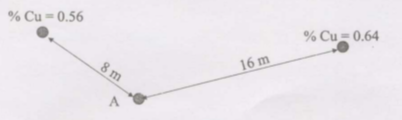
\includegraphics[width=0.6\textwidth]{Screenshot_2025_0812_201406.png}                 
\caption{}
	\label{fig:Q84&Q85}
\end{figure}

\item The grade of copper (\%) at point A using the inverse distance weighting method is  
	\hfill (GATE MN 2007)
\begin{enumerate}
		\begin{multicols}{4}
\item 0.47
\item 0.58
\item 0.61
\item 1.20
	\end{multicols}
\end{enumerate}

\item Assume the grade at A to be the average grade of copper, mill recovery is $90\%$ and the smelting \& refining losses to be $1.0 \ \mathrm{kg}$ of copper per tonne of ore. The saleable copper in kg/tonne of ore is  
	\hfill (GATE MN 2007)
\begin{enumerate}
\begin{multicols}{4}
\item 2.93
\item 3.93
\item 4.93
\item 5.93
	\end{multicols}
\end{enumerate}




\end{enumerate}
\begin{center}                                  
\huge{END OF THE QUESTION PAPER}    
\end{center}

\end{document}

